\documentclass[article]{jss}
\usepackage[utf8]{inputenc}

\providecommand{\tightlist}{%
  \setlength{\itemsep}{0pt}\setlength{\parskip}{0pt}}

\author{
Earo Wang\\Monash University \And Dianne Cook\\Monash University \And Rob J Hyndman\\Monash University
}
\title{Calendar-based graphics for visualising people's daily schedules}

\Plainauthor{Earo Wang, Dianne Cook, Rob J Hyndman}
\Plaintitle{Calendar-based graphics for visualising people's daily schedules}

\Abstract{
This paper describes a \code{frame\_calendar} function that organises
and displays temporal data, collected on sub-daily resolution, into a
calendar layout. Calendars are broadly used in society to display
temporal information, and events. The \code{frame\_calendar} utilizes
linear algebra on the date variable to create the layout. It utilizes
the grammar of graphics to create the plots inside each cell, and thus
synchronises neatly with \pkg{ggplot2} graphics. The motivating
application is studying pedestrian behavior, based on counts which are
captured at hourly interval by sensors scattered around the city.
Facetting by the usual features such as day and month, was not
sufficient to examine the behaviour. Making displays on a monthly
calendar format helps to understand pedestrian patterns relative to
events such as work days, weekends, holidays, and special events. The
layout algorithm has several format variations and options. It is
implemented in the R package \pkg{sugrrants}.
}

\Keywords{data visualisation, statistical graphics, time series, R package, grammar of graphics}
\Plainkeywords{data visualisation, statistical graphics, time series, R package, grammar of graphics}

%% publication information
%% \Volume{50}
%% \Issue{9}
%% \Month{June}
%% \Year{2012}
%% \Submitdate{}
%% \Acceptdate{2012-06-04}

\Address{
    Earo Wang\\
  Monash University\\
  Department of Econometrics and Business Statistics, Monash University,
  VIC 3800 Australia\\
  E-mail: \email{earo.wang@monash.edu}\\
  
      Dianne Cook\\
  Monash University\\
  Department of Econometrics and Business Statistics, Monash University,
  VIC 3800 Australia\\
  E-mail: \email{dicook@monash.edu}\\
  
      Rob J Hyndman\\
  Monash University\\
  Department of Econometrics and Business Statistics, Monash University,
  VIC 3800 Australia\\
  E-mail: \email{rob.hyndman@monash.edu}\\
  
  }

\usepackage{amsmath}

\begin{document}

\section{Introduction}\label{introduction}

This work was originally motivated by studying foot traffic in the city
of Melbourne \citep{ped}. There have been 43 installed sensors counting
pedestrians every hour across the downtown area until the end of 2016
(see Figure \ref{fig:ped-map}). The dataset can shed lights into
understanding people's daily schedules, or assisting administration and
business planning. We start off with the conventional time series plot
to catch a glimpse of such data. A small multiples, shown in Figure
\ref{fig:time-series-plot}, gives an overall picture of foot traffic at
a selection of 3 sensors. Figure \ref{fig:facet-time} provides another
aspect of temporal patterns in the more detailed level by faceting day
of the week. It lends itself to a number of issues that make exploratory
data visualisation challenging in many temporal-context applications
involving human behaviours:

\begin{enumerate}
\def\labelenumi{\arabic{enumi}.}
\tightlist
\item
  Variations primarily result from multiple time scales including time
  of day, day of week, and day of year (such as public holiday and
  recurred events).
\item
  Since the data are often collected at daily frequency or a time scale
  more frequent than daily, they typically involve a large number of
  observations spanning over a long time period.
\item
  Measurements of a single type are made at multiple locations at a
  given time point, which creates the need in comparing and contrasting
  between locations.
\end{enumerate}

\begin{CodeChunk}
\begin{figure}

{\centering 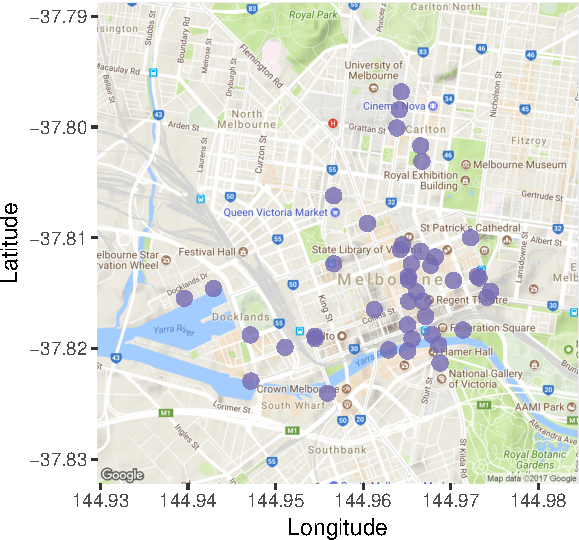
\includegraphics[width=0.55\linewidth]{figure/ped-map-1} 

}

\caption[Map of the Melbourne city with purple dots indicating sensor locations]{Map of the Melbourne city with purple dots indicating sensor locations.}\label{fig:ped-map}
\end{figure}
\end{CodeChunk}

\begin{CodeChunk}
\begin{figure}

{\centering 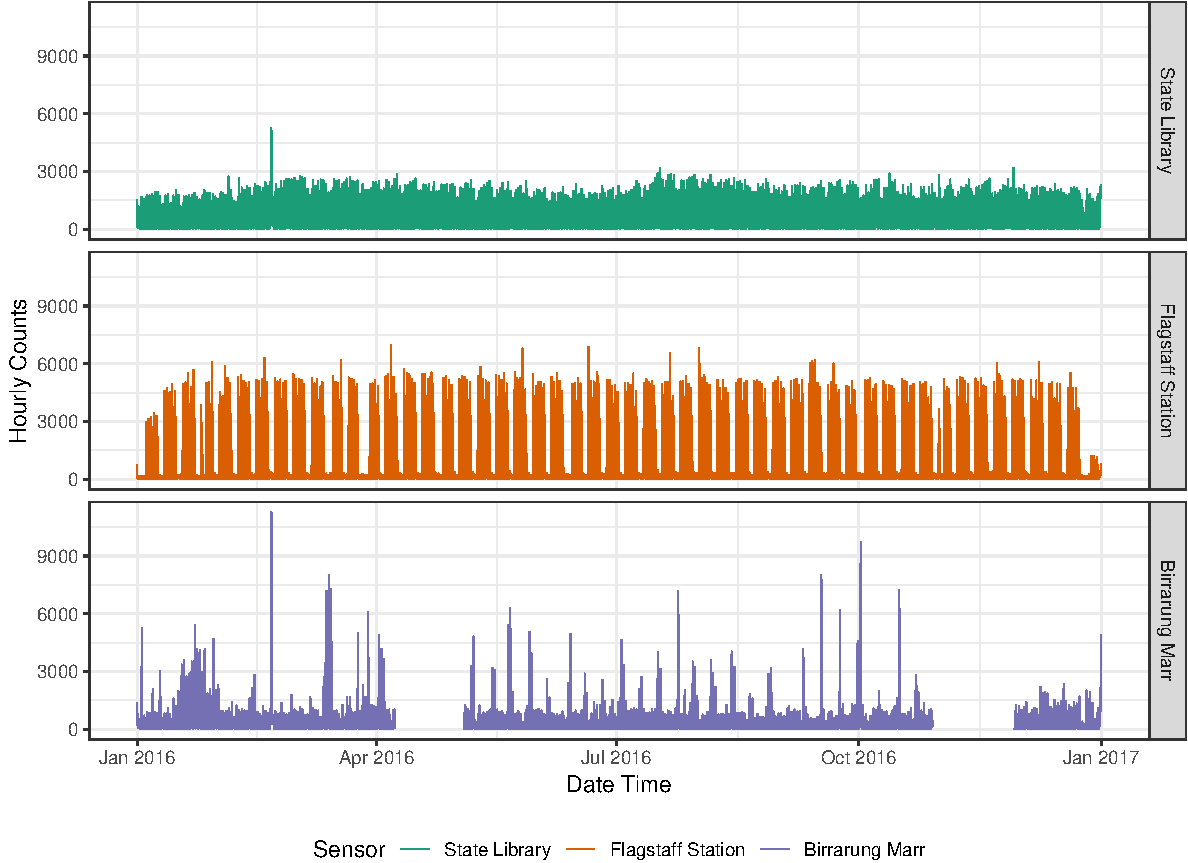
\includegraphics[width=\textwidth]{figure/time-series-plot-1} 

}

\caption[Time series plot about the number of pedestrians over the year of 2016 at a selection of 3 sensors in the city of Melbourne]{Time series plot about the number of pedestrians over the year of 2016 at a selection of 3 sensors in the city of Melbourne. Coloured by the sensors, small multiples of lines show that the foot traffic varies from one sensor to another in terms of both time and number. The weekly patterns look distincitve across these 3 sensors. There is an eye-catching spike occurred to State Library, which is caused by the annual event--White Night--on 20th of Feburary.}\label{fig:time-series-plot}
\end{figure}
\end{CodeChunk}

\begin{CodeChunk}
\begin{figure}

{\centering 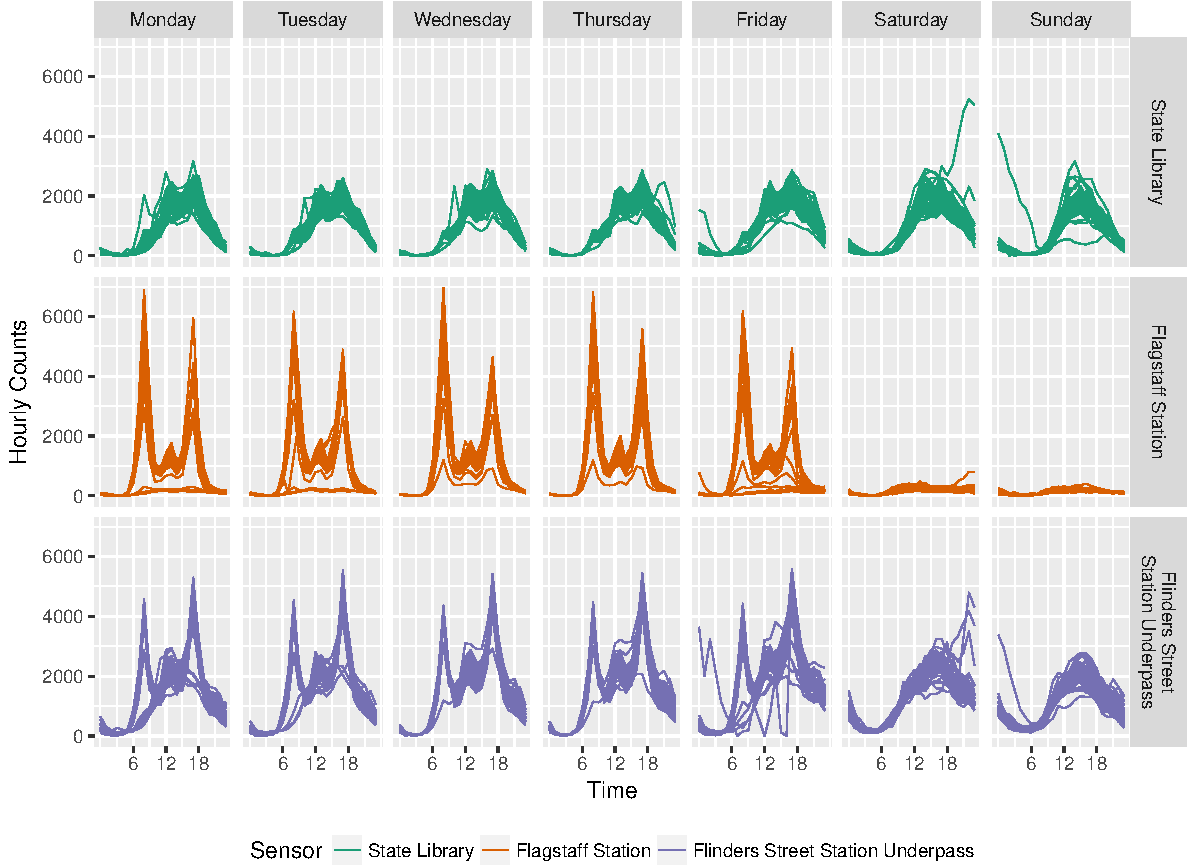
\includegraphics[width=\textwidth]{figure/facet-time-1} 

}

\caption[Hourly pedestrian counts facetted by sensors and days of the week using lines]{Hourly pedestrian counts facetted by sensors and days of the week using lines. It features at least two types of seasons--time of day and day of week--across all the sensors. The temporal patterns are subject to the sensor locations too.}\label{fig:facet-time}
\end{figure}
\end{CodeChunk}

A collection of data plots, organised in a familiar format, offer a
useful and intuitive way to tell a richer story and reveal more complex
relationships. \citet{Wickham2012glyph} embedded a sequence of daily
temperature line charts into a glyph map according to the spatial
locations; and \citet{R-geofacet} provided methods to arrange the data
plots of many types into a preserved geographical grid in the
\pkg{geofacet} package. They both attempt to have the self-contained
data plots in spatial context.

Alternatively, calendar-based graphics turn out to be a useful tool in
unfolding human-related activities in temporal context. For example,
\citet{VanWijkCluster1999} developed a calendar view of heatmap to
represent the number of employees in the work place over a year, where
colours indicate different clusters derived from the days. It contrasts
weekdays and weekends, highlights public holiday, and presents other
known seasons like school vacations, all of which have influence over
the turn-outs in the office. The calendar-based heatmap was implemented
in a couple of R packages: \pkg{ggTimeSeries} \citep{R-ggTimeSeries} and
\pkg{ggcal} \citep{R-ggcal}. However, these techniques are too
constrained to colour-encoding graphics and day of week as the smallest
time scale. Time of day, which serves as one of the most important
aspect in explaining variations arisen from pedestrian sensor data, will
be neglected through daily aggregation. Additionally if simply using
coloured blocks rather than curves, it may become perceptually difficult
to estimate the shape positions and changes, although using the curves
comes with the cost of more display capacity
\citep{cleveland1984graphical, lam2007overview}.

We propose a new algorithm via linear algebra tools to go beyond the
calendar-based heatmap. The approach is developed with these conditions
in mind: (1) to make time of day present in addition to the existing
temporal components such as day of week and day of year, (2) to
incorporate line graphs and other types of glyphs into the graphical
toolkit for the calendar layout, (3) to enable an overlaying plot
consisting of multiple time series. The proposed algorithm has been
implemented to the \code{frame_calendar} function in the \pkg{sugrrants}
package \citep{R-sugrrants} using \proglang{R} \citep{R-base}.

The remainder of the paper is organised as follows. Section
\ref{sec:algorithm} demonstrates the construction of the calendar layout
in depth. Section \ref{sec:opt} lists and describes the options that
come with the \code{frame_calendar} function. Section \ref{sec:examples}
presents some variations of its usage. Section \ref{sec:discussion}
discusses the advantages and disadvantages of the method.

\section{Construction}\label{construction}

\label{sec:algorithm}

Figure \ref{fig:flinders-2016} shows the line glyphs framed in the
monthly calendar over the year of 2016. This is achieved by the
\code{frame_calendar} function computing the new coordinates according
to the input data variables; in turn the rearranged data values are
plotted using the \pkg{ggplot2} package \citep{R-ggplot2}, which is the
implementation of the grammar of graphics
\citep{wilkinson2006grammar, wickham2010layered}.

\begin{CodeChunk}
\begin{figure}

{\centering 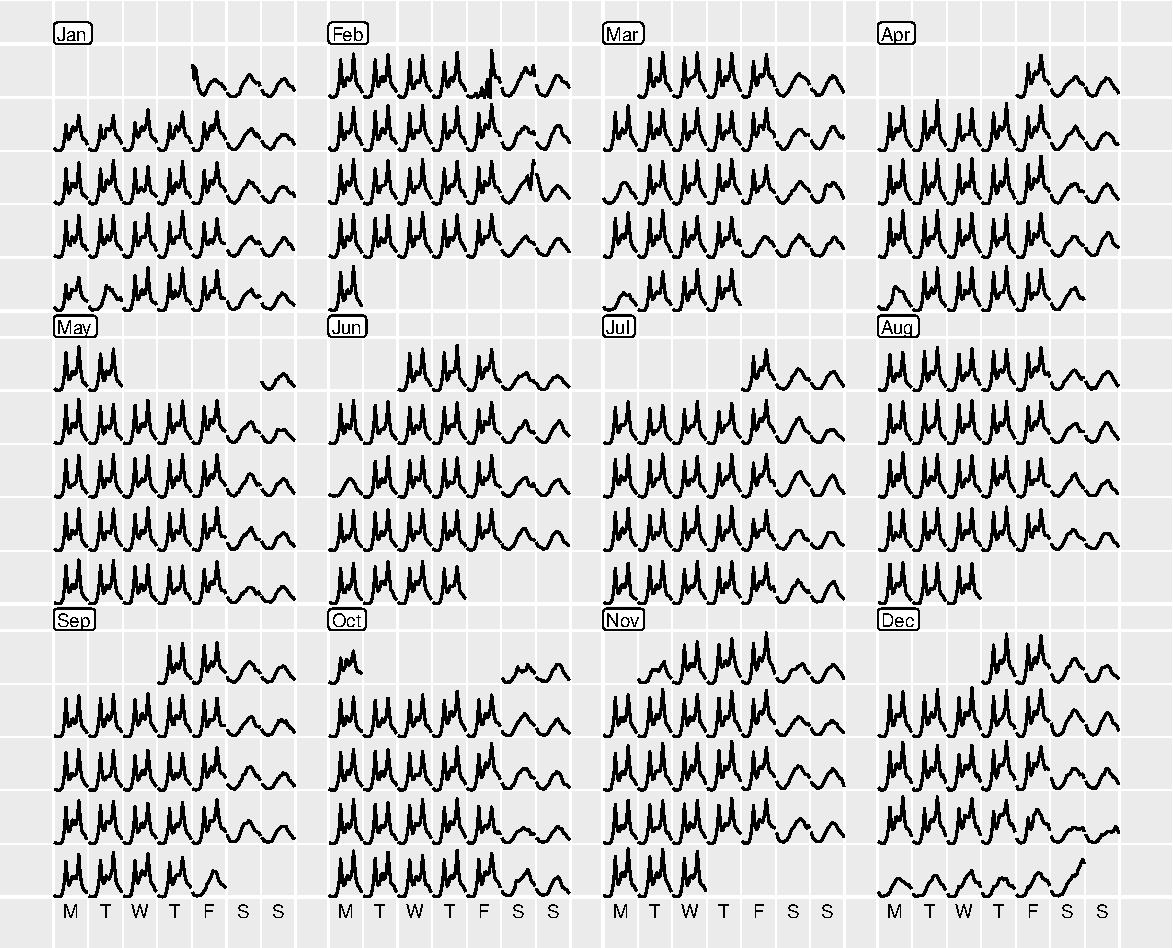
\includegraphics[width=\textwidth]{figure/flinders-2016-1} 

}

\caption[The calendar-based display of hourly foot traffic at Flinders Street Station using line glyphs]{The calendar-based display of hourly foot traffic at Flinders Street Station using line glyphs. The arrangement of 3 by 4 on the monthly calendar format presents all the traffic in 2016. The disparities between weekday and weekend along with public holiday pop out to viewers in the clearer manner.}\label{fig:flinders-2016}
\end{figure}
\end{CodeChunk}

The algorithm for constructing a calendar plot uses linear algebra,
similar to that used in the glyph map displays for spatio-temporal data
\citep{Wickham2012glyph}. To make a year long calendar, requires cells
for days, embedded in blocks corresponding to months, organised into a
grid layout for a year. Each month can be captured with 35 (5 \(\times\)
7) cells, where the top left is Monday of week 1, and the bottom right
is Sunday of week 5. These cells provide a micro canvas on which to plot
the data. The first day of the month could be any of Monday-Sunday,
which is determined by the year of the calendar. Months are of different
length days, ranging form 28-31, and each month could extend over six
weeks but the convention in these months is to wrap the last few days up
to the top row of the block. The notation for creating these cells is as
follows:

\begin{itemize}
\tightlist
\item
  \(k = 1, \dots , 7\) is the day of the week that is the first day of
  the month.
\item
  \(d = 28, 29, 30\) or \(31\) representing the number of days in any
  month.
\item
  \((i, j)\) is the grid position where \(1 \le i \le 5\) is week within
  the month, \(1 \le j \le 7\), is day of the week.
\item
  \(g = k, \dots,(k+d)\) indexes the day in the month, inside the 35
  possible cells.
\end{itemize}

The grid position for any day in the month is given by

\begin{equation}
  \begin{aligned}
  i &= \lceil (g \mod 35) / 7\rceil, \\
  j &= g \mod 7. \label{eq:grid}
  \end{aligned}
\end{equation}

Figure \ref{fig:month-diagram} illustrates this \((i,j)\) layout for a
month where \(k=5\).

\begin{CodeChunk}
\begin{figure}

{\centering 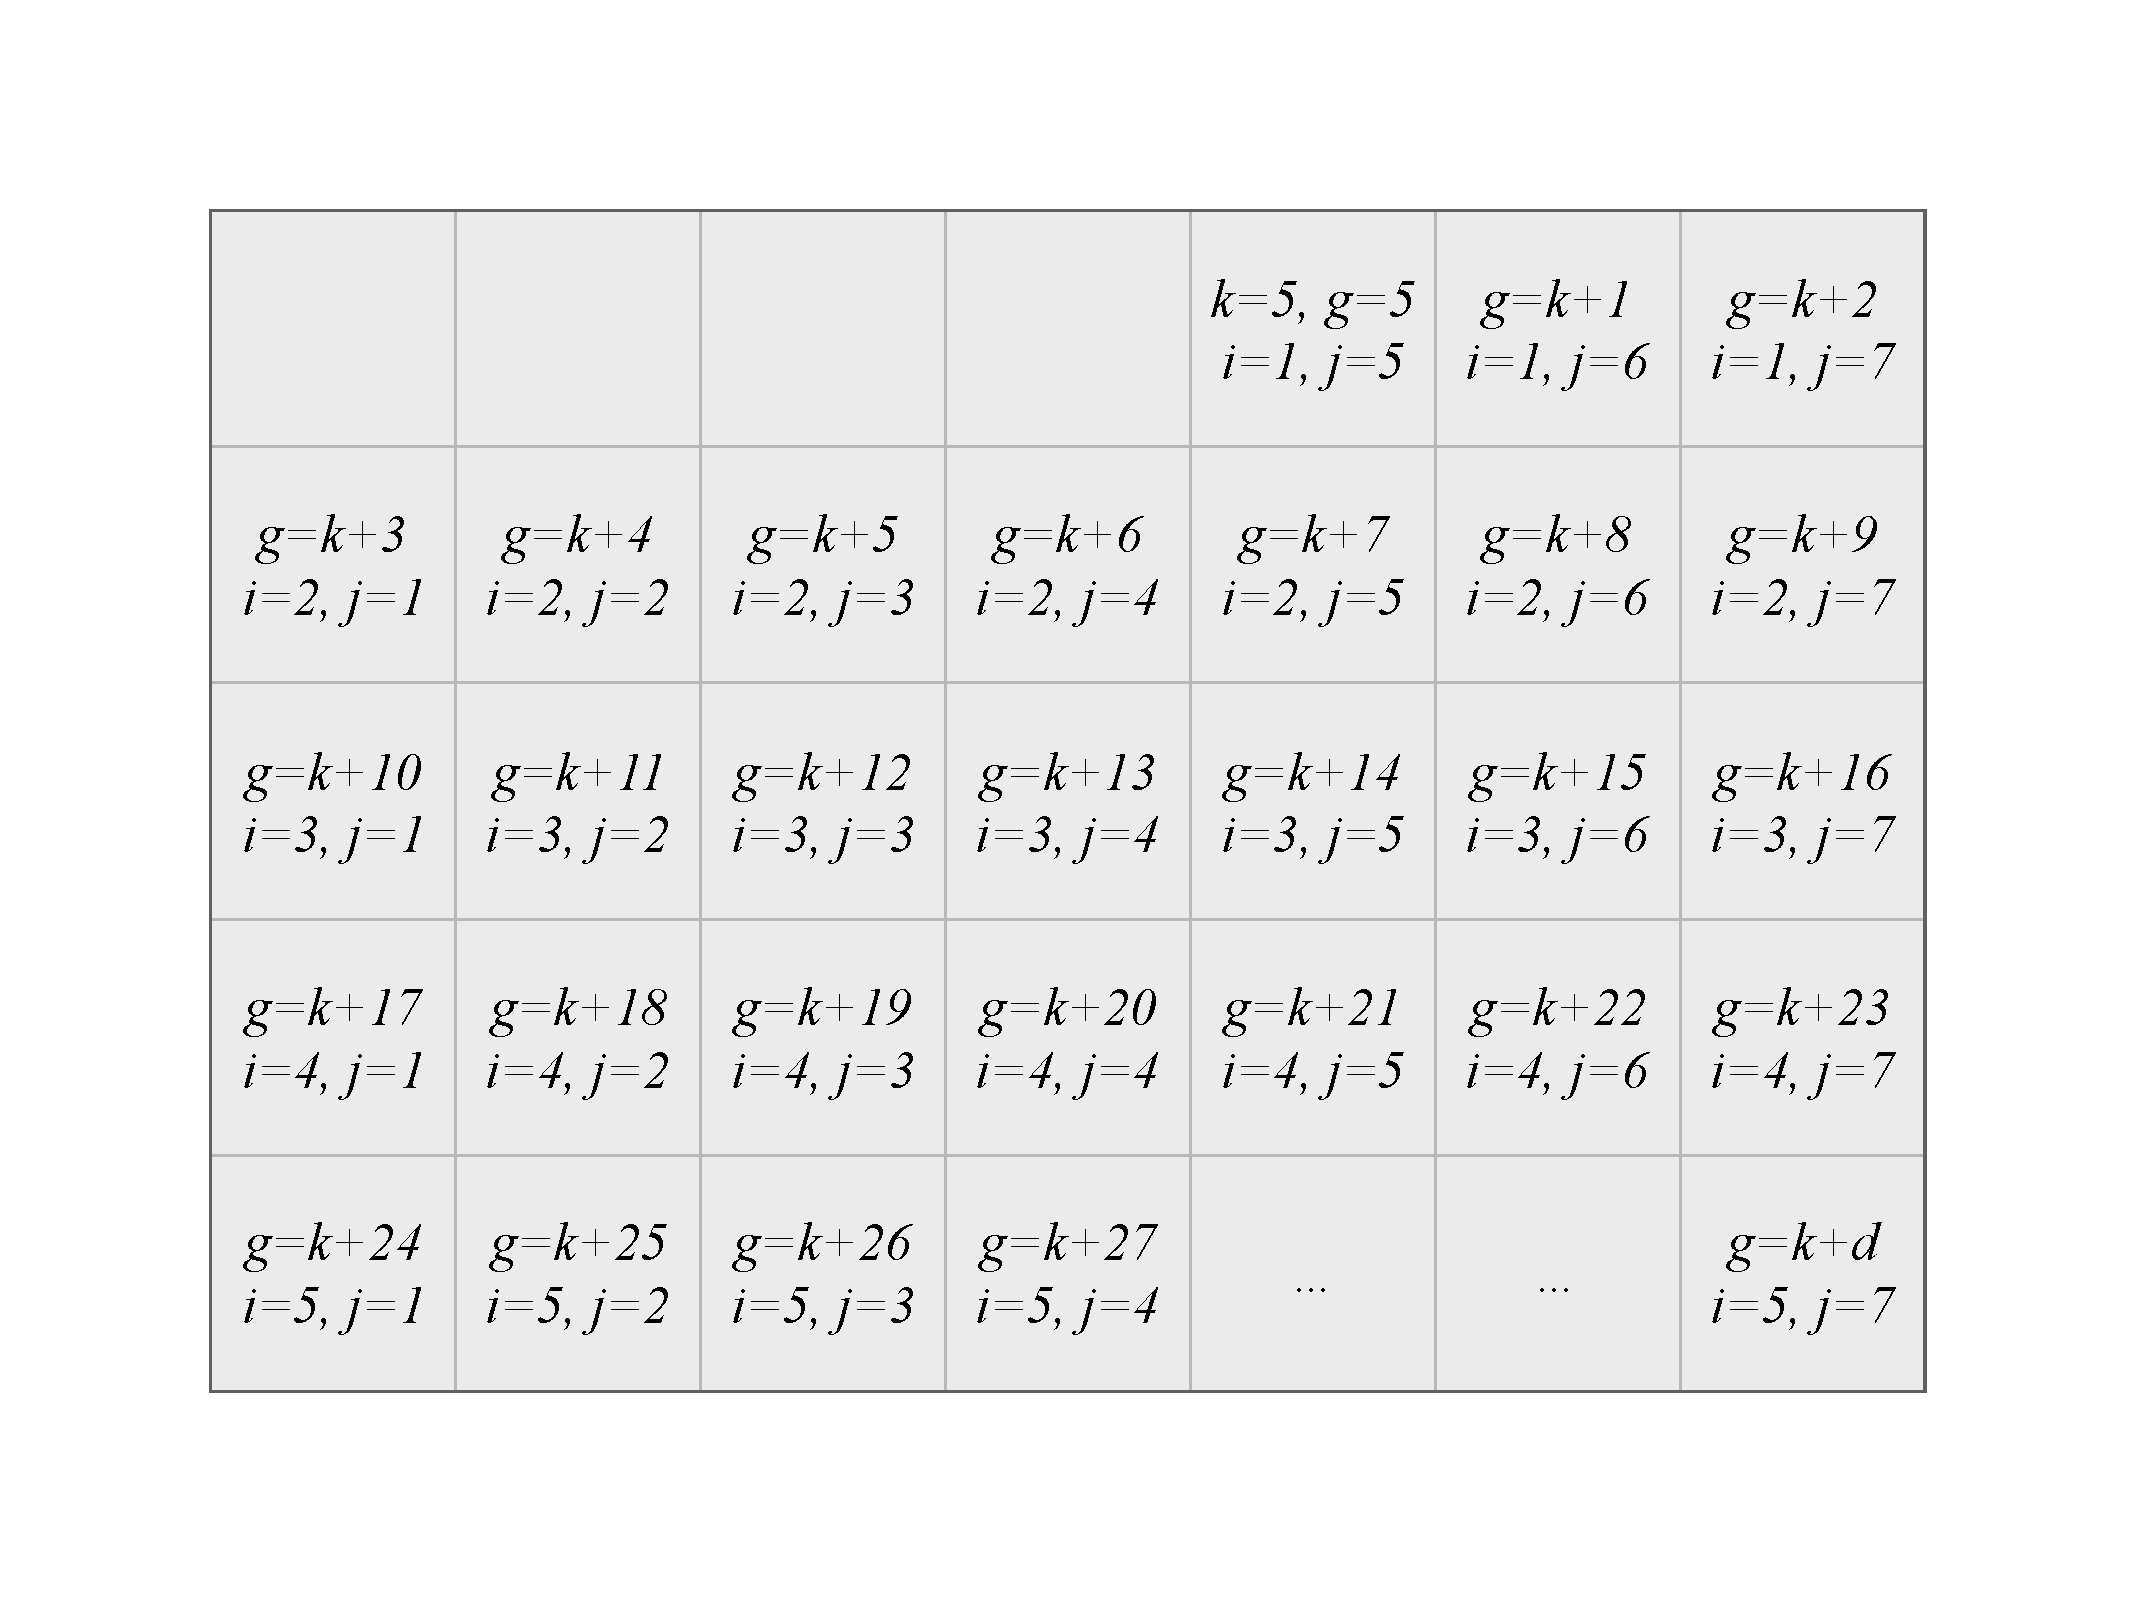
\includegraphics[width=360pt,height=250pt]{figure/month} 

}

\caption[Illustration of the indexing layout for cells in a month]{Illustration of the indexing layout for cells in a month.}\label{fig:month-diagram}
\end{figure}
\end{CodeChunk}

To create the layout for a full year, \((m, n)\) denotes the position of
the month arranged in the plot, where \(1 \le m \le M\) and
\(1 \le n \le N\). Between each month requires some small amount of
white space, label this \(b\). Figure \ref{fig:year-diagram} illustrates
this layout.

\begin{CodeChunk}
\begin{figure}

{\centering 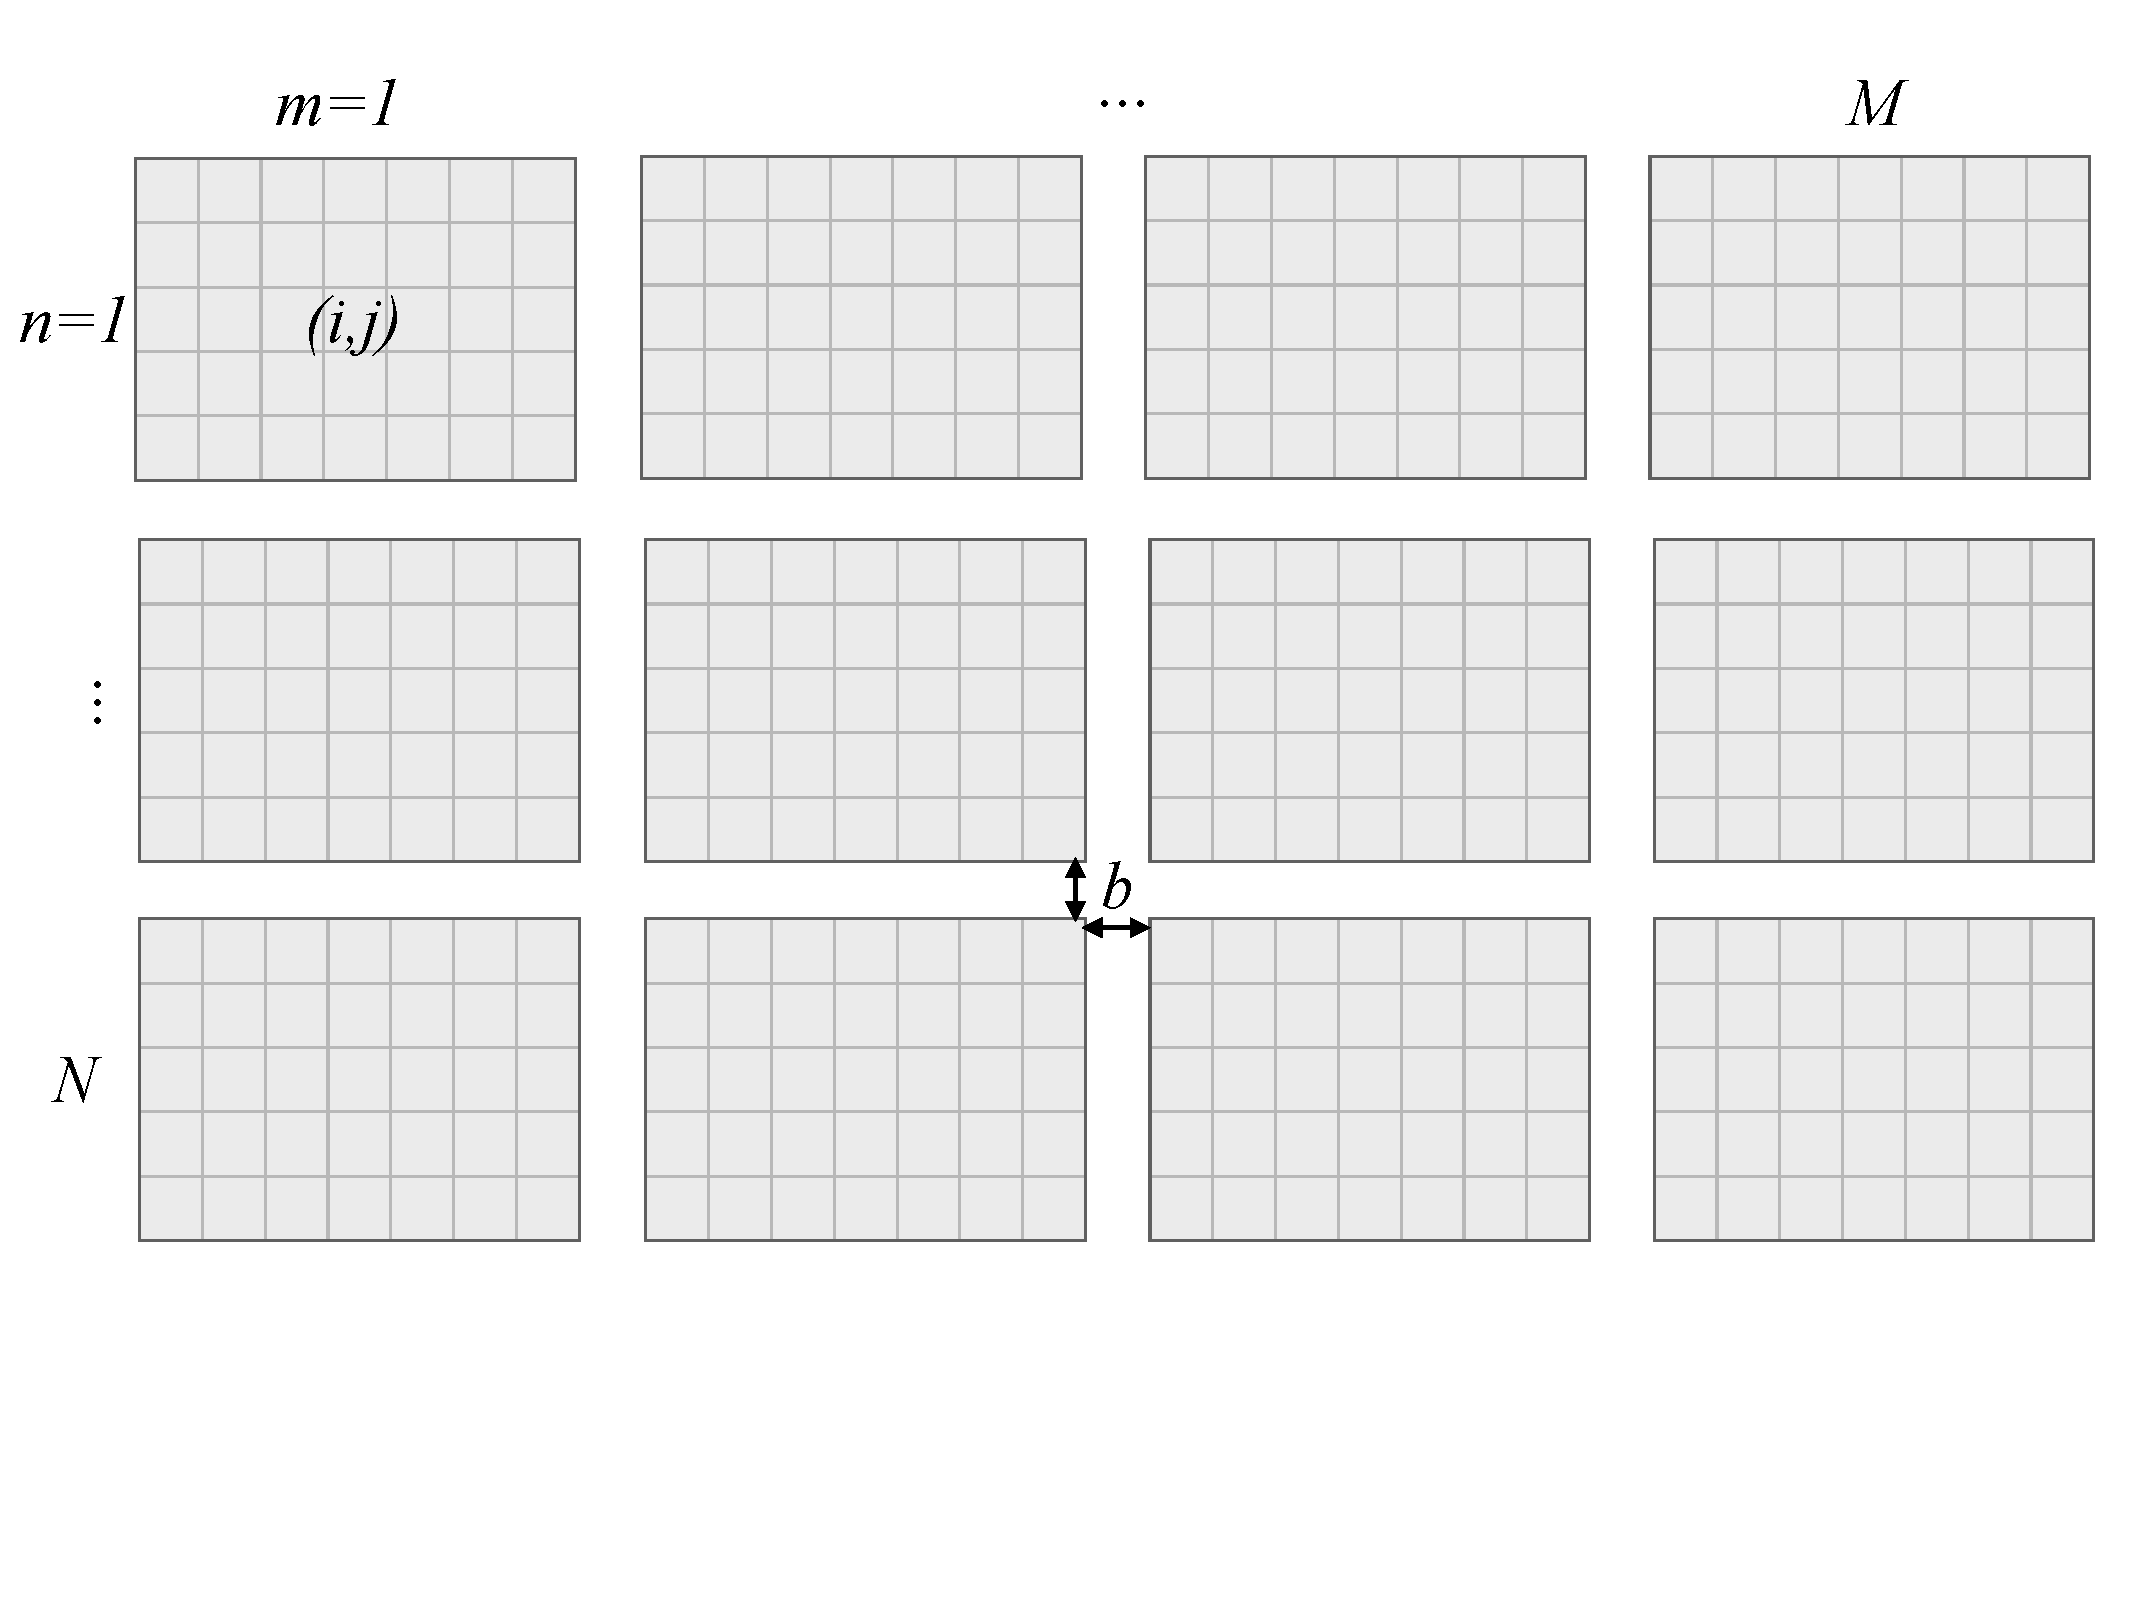
\includegraphics[width=360pt,height=250pt]{figure/year} 

}

\caption[Illustration of the indexing layout for months of one year]{Illustration of the indexing layout for months of one year.}\label{fig:year-diagram}
\end{figure}
\end{CodeChunk}

Each cell forms a canvas on which to draw the data. Consider the canvas
to have limits \([0, 1]\) horizontally and vertically. For the
pedestrian sensor data, within each cell hour is plotted horizontally
and count is plotted vertically. Each variable is scaled to have values
between \([0,1]\), using the minimum and maximum of all the data values
to be displayed assuming of fixed scales. Let \(h\) be the scaled hour,
and \(c\) the scaled count.

Then the final points for making the calendar line plots of the
pedestrian sensor data is given by:

\begin{equation}
  \begin{aligned}
  x &= i + (i - 1) \times m + (m - 1) \times b + h, \\
  y &= -j - (j - 1) \times n - (n - 1) \times b + c. \label{eq:final}
  \end{aligned}
\end{equation}

Note that for the vertical direction, the top left is the starting point
of the grid, hence the subtractions, and resulting negative values to
lay out the cells. Within each cell, the starting position is bottom
left.

The algorithm can be relatively easily extended to layout from a single
month to a few years, based on the period of time to be visualised.
\((M, N)\) can be determined by the user using the arguments of
\code{nrow} and \code{ncol}. If the one would like to visualise data
spanning over three years, for example, \(M = 12\) and \(N = 3\) seem to
be an appropriate choice when assessing the differences of a given month
across the years.

We only illustrate that grids are laid out over the horizontal direction
in the paper. The vertical direction can be enabled by swapping \(i\)
and \(j\) in the algorithm stated above when the argument \code{dir} is
set to \code{"v"}. It particularly benefits those users who get
accustomed to calendars of vertical organisation in some countries.

\section{Options}\label{options}

\label{sec:opt}

There are a few options provided for the \code{frame_calendar} function
to adjust the display and they are shown as follows:

\begin{verbatim}
frame_calendar(
  data, x, y, date, calendar = "monthly", dir = "h", sunday = FALSE, 
  nrow = NULL, ncol = NULL, polar = FALSE, scale = "fixed",
  width = 0.95, height = 0.95
)
\end{verbatim}

Assuming that tidy data \citep{wickham2014tidy} is the underlining data
structure, the \code{x} takes a variable that will be mapped to the x
axis and the \code{y} mapped to the y axis for the later plotting. In
Figure \ref{fig:flinders-2016}, for example, the \code{x} is the
variable specifying the time of the day, and the \code{y} is the
variable suggesting the hourly counts. The \code{date} argument is given
by the date variable that determines the correct order in the calendar
layout. We shall describe some of the arguments that allow for different
displays.

\subsection{Layouts}\label{layouts}

The algorithm described in Section \ref{sec:algorithm} is for the most
common calendar layout--``monthly'' calendar, and it can be simplified
to accommodate the other two types of calendar formats. One is comprised
of days of a week in columns and weeks of a year in rows, and the other
is days of a month in columns and months of a year in rows, which we
refer to as ``weekly'' and ``daily'' calendar respectively. Which layout
to be used is controlled by the \code{calendar} argument. Due to the way
of the arrangement, the weekly calendar puts more emphases on days of a
week over days of a year, whereas the daily one serves as the opposite.
The monthly format can be considered as the advanced twist of both
weekly and daily. Temporal patterns lead to which format to be employed.
The weekly calendar can be a nice attempt if the most variations can be
characterised by days of a week. On the other hand, the absence of
weekly effect but the presence of yearly effect can direct to the daily
calendar. When both are present, the monthly calendar appears to be a
better choice.

\subsection{Polar transformation}\label{polar-transformation}

When \code{polar = TRUE}, the polar transformation is carried out for
the data. Again the computation remain similar to the one described in
\citet{Wickham2012glyph}. Figure \ref{fig:flinders-polar} is considered
as the spiral display of Figure \ref{fig:flinders-2016}.

\begin{CodeChunk}
\begin{figure}

{\centering 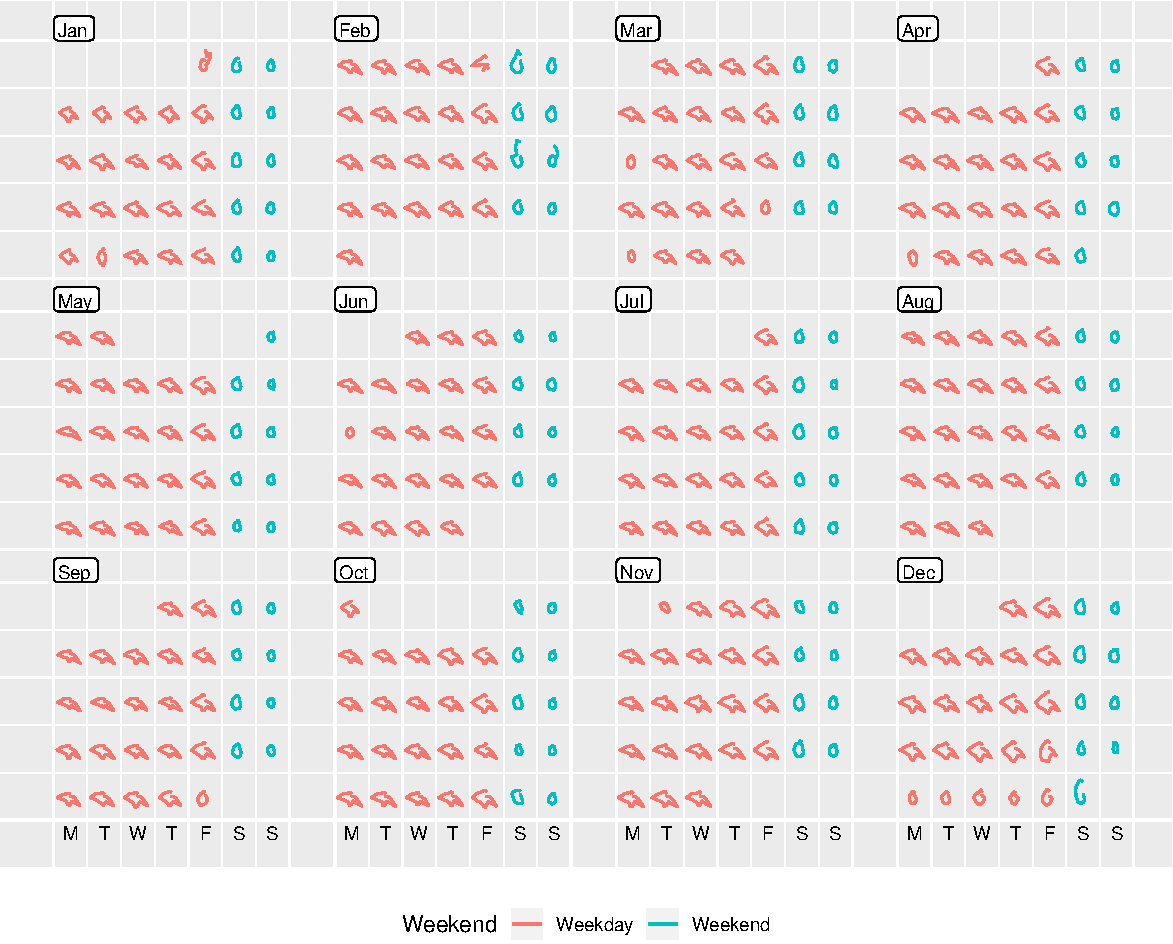
\includegraphics[width=\textwidth]{figure/flinders-polar-1} 

}

\caption[Star plots of hourly pedestrian counts at Flinders Street Station, which are line charts placed in polar coordinates]{Star plots of hourly pedestrian counts at Flinders Street Station, which are line charts placed in polar coordinates. The periodic behaviours on workdays are clearly visible.}\label{fig:flinders-polar}
\end{figure}
\end{CodeChunk}

\subsection{Scales}\label{scales}

Section \ref{sec:algorithm} discusses the implementation applied to the
fixed scale which is using the whole range of all the data values. The
\code{scale} argument controls the scaling of the display. The fixed
scale (\code{fixed}) is the default, meaning the data values in all
positions to be scaled. The remaining options include free scale within
each cell (\code{free}), cells derived from the same day of the week
(\code{free_wday}), or cells from the same day of the month
(\code{free_mday}). It utilises the comparisons of absolute or relative
values, and the emphases of various types of variations.

Grouping the cells based on the same time period gives rise to the
different scales. For example, the minimums and maximums obtained from
each cell, that is every day \((i, j)\) together with \((m, n)\), result
in local scale. The overall variation gives way to the individual shape.
Figure \ref{fig:flinders-free} is an example of plotting line charts
scaled locally. The daily variation is made more distinctive, compared
to Figure \ref{fig:flinders-2016}.

Similarly, the same \(j\) indexing day of the week is grouped to compute
the scales in days of a week; in other words, the same value within a
given \(j\) corresponds to the same position across each
\(j\)\textsuperscript{th} cell. To construct the scales for days of the
month, \(g\) representing day of the month is used. This makes it easier
to compare shape of a given day across each month block. The scaling
option combined with the calendar layouts offers a number of varieties
to construct the plot.

\begin{CodeChunk}
\begin{figure}

{\centering 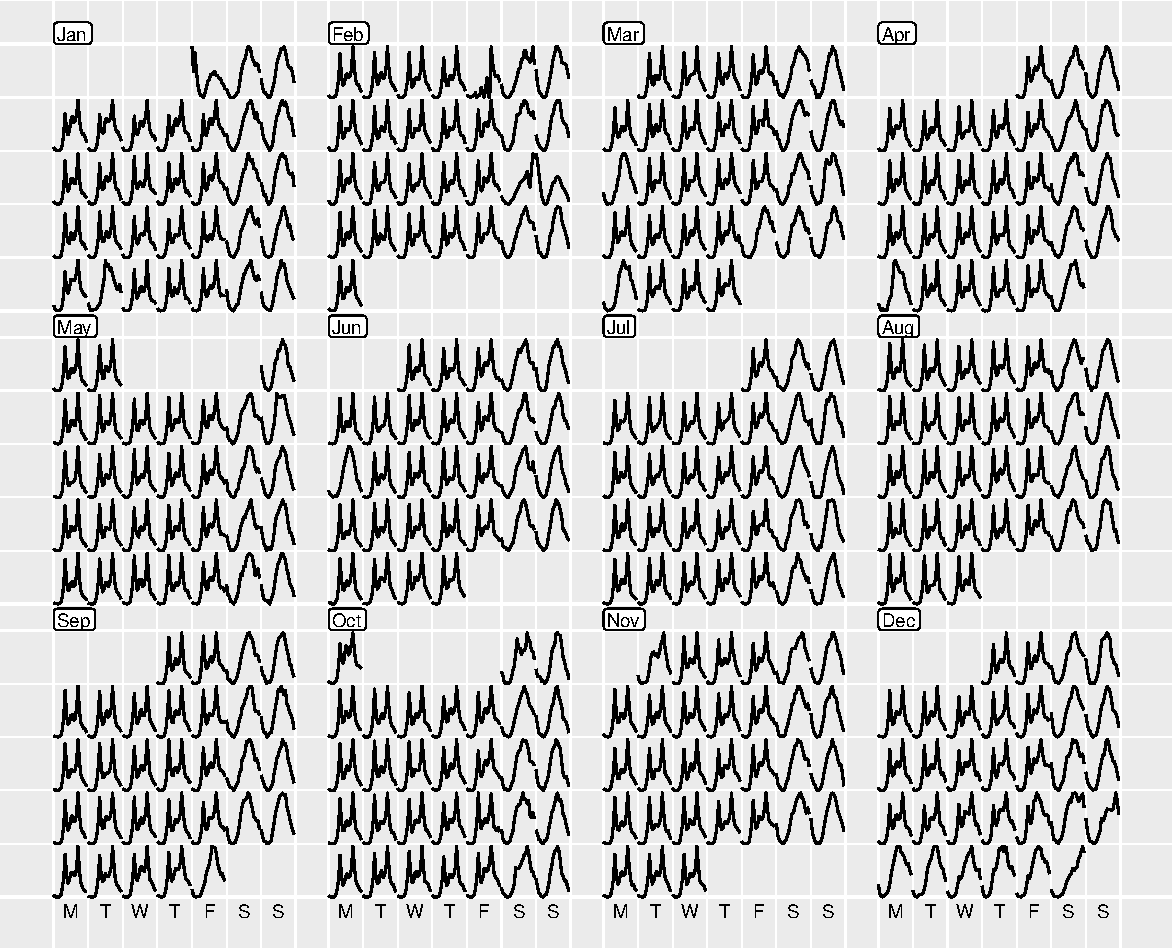
\includegraphics[width=\textwidth]{figure/flinders-free-1} 

}

\caption[Line glyphs on the calendar format showing hourly foot traffic at Flinders Street Station, scaled over all the days]{Line glyphs on the calendar format showing hourly foot traffic at Flinders Street Station, scaled over all the days. The individual shape on a single day becomes more distinctive at the expense of the magnitude comparison loss.}\label{fig:flinders-free}
\end{figure}
\end{CodeChunk}

\subsection{Reference lines and
labels}\label{reference-lines-and-labels}

Reference lines dividing each cell and block as well as labels
indicating weekday and month are also provided in order to make
calendar-based graphics more accessible and informative.

Regarding the monthly calendar, the major reference lines separate every
month panel and the minor ones separate every cell, represented by the
thick and thin lines respectively. The major reference lines are placed
surrounding every month block: for each \(m\), the vertical lines are
determined by \(\min{(x)}\) and \(\max{(x)}\); for each \(n\), the
horizontal lines are given by \(\min{(y)}\) and \(\max{(y)}\). The minor
reference lines are placed on the left side of every cell: for each
\(i\), the vertical division is \(\min{(x)}\); for each \(j\), the
horizontal is \(\min{(y)}\).

The abbreviated month labels located on the top left are obtained
through \((\min{(x)}, \max{(y)})\) for every \((m, n)\). The weekday
texts with a single letter are uniformly positioned on the bottom of the
whole canvas, that is \(\min{(y)}\), with the central position of a cell
\(x / 2\) for each \(j\).

\section{Variations}\label{variations}

\label{sec:examples}

\subsection{Overlaying and faceting
subsets}\label{overlaying-and-faceting-subsets}

The comparison of one sensor to another adds additional insights to the
dataset, which is commonly done with an overlaying plot such as Figure
\ref{fig:overlay}. For instance, the dominant patterns occurred to both
train stations--Flinders Street Station and Flagstaff station--are
together driven by the commuters on the work days; however, the former
is much outnumbered than the latter during the weekends and public
holidays. It suggests that Flagstaff station limits its functionality as
simply the public transport hub for day-to-day commuters, but various
activities take place around the Flinders Street Station other than
commuting. Because Flinders Street Station closely lies to South Bank
and other places of attractions where the locals go for leisure and the
tourists for travelling. It can be noted from Figure \ref{fig:overlay}
that State Library follows the similar temporal trend as Flinders Street
Station on non-work days. The nighttime events, such as White Night and
New Year Evening Firework, has barely affected the operation of
Flagstaff Station but heavily affected the incoming and outgoing traffic
to Flinders Street Station and State Library on these days.

\begin{CodeChunk}
\begin{figure}

{\centering 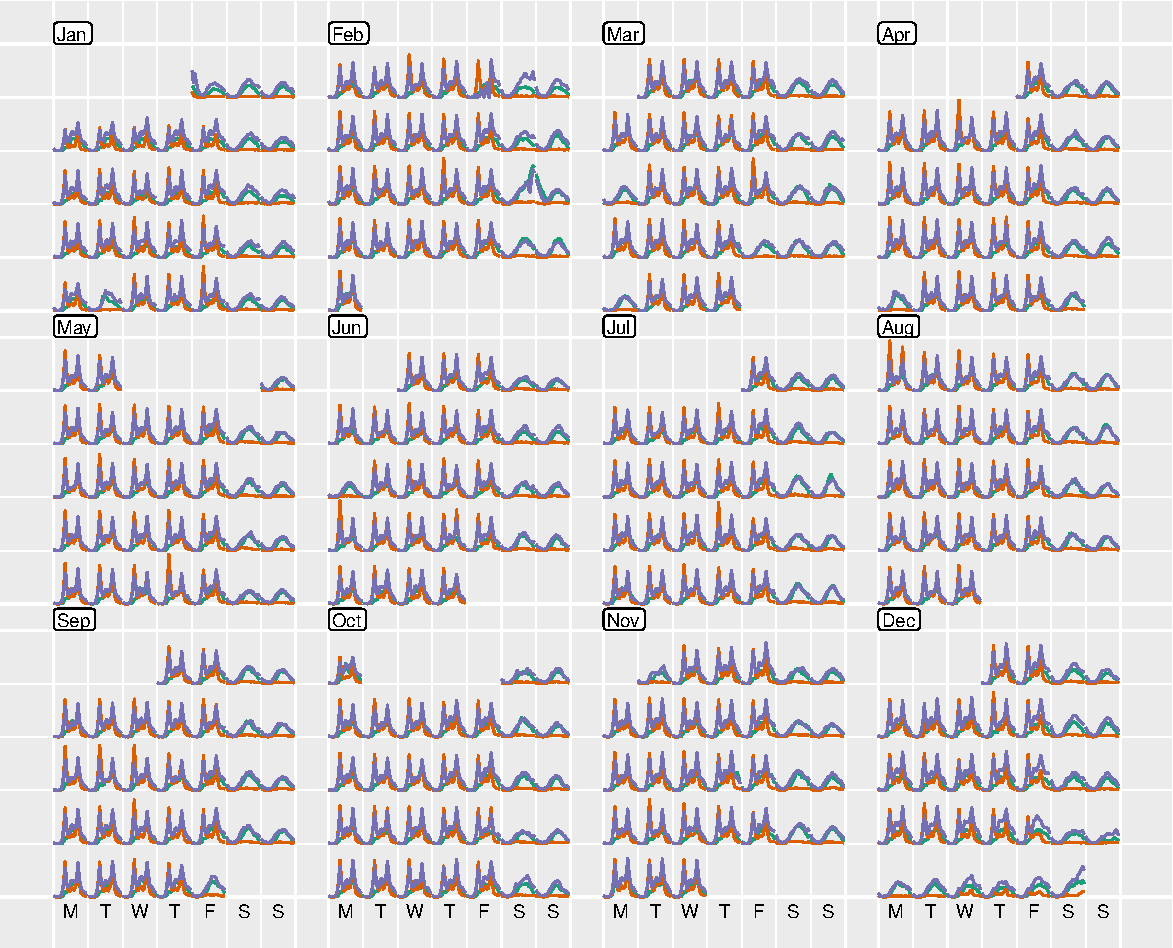
\includegraphics[width=\textwidth]{figure/overlay-1} 

}

\caption[Overlaying line graphs of the 3 sensors in the monthly calendar]{Overlaying line graphs of the 3 sensors in the monthly calendar. Flagstaff station is not as busy as the other two on non-work days.}\label{fig:overlay}
\end{figure}
\end{CodeChunk}

Placing multiple series on the common scale makes the magnitudes
comparable between them; the glyphs are yet small in size, resulting in
the overlapping problem. To avoid the problem, the calendar layout can
be embedded into a series of plots for the different sensors. Figure
\ref{fig:facet} presents the idea of the graphs of calendar plots. By
doing so, the comparability with respect to the magnitudes is sacrificed
for the emphasis of the individual sensor.

\begin{CodeChunk}
\begin{figure}

{\centering 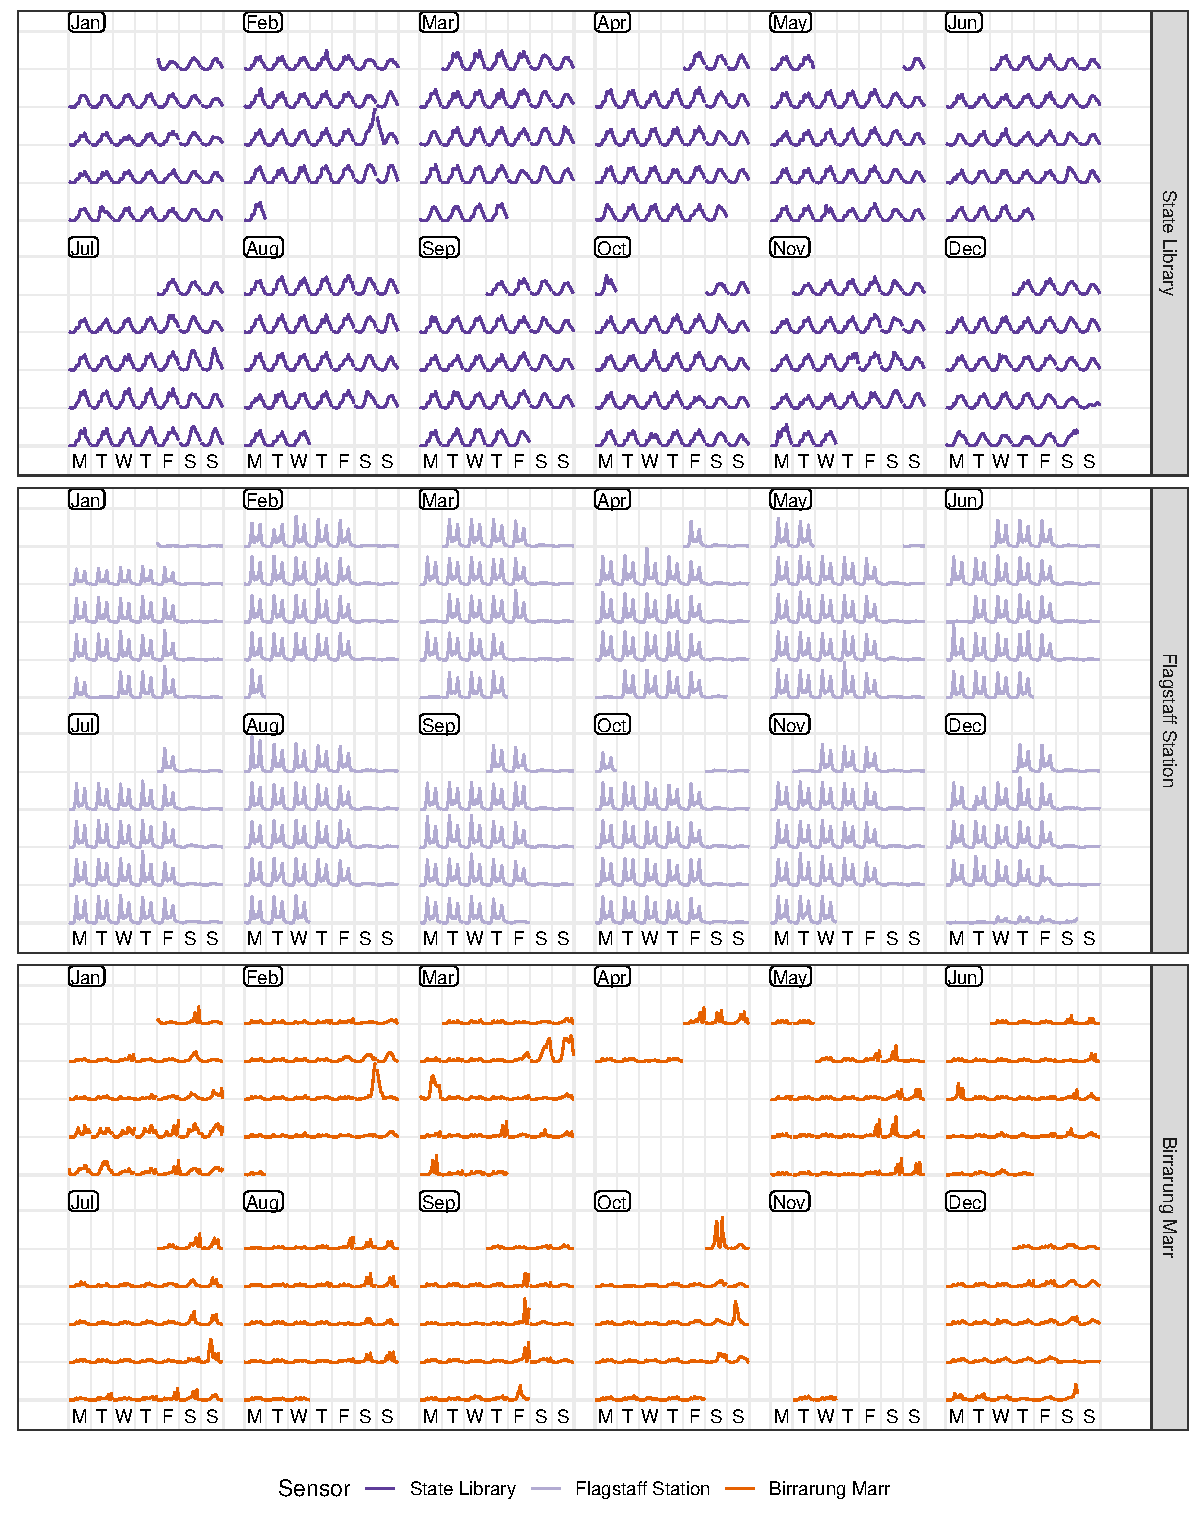
\includegraphics[width=\textwidth]{figure/facet-1} 

}

\caption[Line charts, embedded in the 6 by 2 monthly calendar, coloured and faceted by the 3 sensors]{Line charts, embedded in the 6 by 2 monthly calendar, coloured and faceted by the 3 sensors. The variations of an individual sensor are emphasised, and the shapes can be compared across the cells and sensors.}\label{fig:facet}
\end{figure}
\end{CodeChunk}

\subsection{Different types of plots}\label{different-types-of-plots}

The \code{frame_calendar} function does not constrain itself to mapping
only temporal variable to the \code{x}. Figure \ref{fig:scatterplot}
shows the lag scatterplot, where the current hourly count is assigned to
the \code{x} and the lagged hourly count to the \code{y} at Flinders
Street Station, organised in the daily calendar. It provides a visual
tool for identifying repeating patterns. Figure \ref{fig:scatterplot}
indicates two separate paths in the work-day glyphs, which suggests that
an hour of a work day with many pedestrians is likely to be followed by
the time of either more pedestrians or fewer. Quite the contrary, the
relationship is so consistent on the non-work days. This is a clear sign
of bimodalily on work days whereas unimodality on the rest of the days,
which is also supported by Figure \ref{fig:flinders-2016}.

\begin{CodeChunk}
\begin{figure}

{\centering 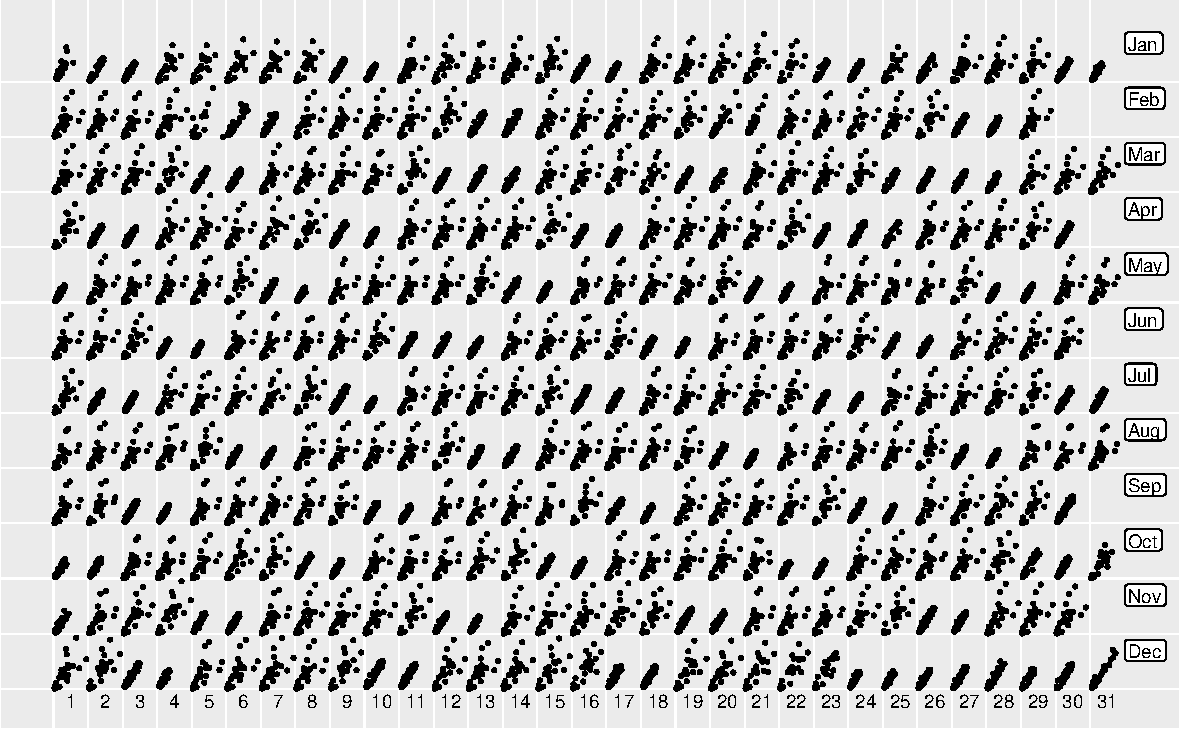
\includegraphics[width=\textwidth]{figure/scatterplot-1} 

}

\caption[Lag scatterplot in the daily calendar layout]{Lag scatterplot in the daily calendar layout. Previous hour's count is plotted against each hour's count at Flinders Street Station to demonstrate the autocorrelation at lag 1. The correlation between them is more consitent on non-work days than work days.}\label{fig:scatterplot}
\end{figure}
\end{CodeChunk}

The newly computed coordinates not only work with the simple geoms such
as lines and points, but also boxplot and other complex geoms. Figure
\ref{fig:boxplot} uses the loess smooth line superimposed atop the
side-by-side boxplots as an example. It shows the distribution of hourly
counts across all the 43 sensors. In general, bimodality features work
days whereas unimodality features the rest of the days. The last week of
December is just the holiday season: people are off work on the day
before Christmas, go shopping on the Boxing day, and hanging out for the
firework in the New Year Evening.

\begin{CodeChunk}
\begin{figure}

{\centering 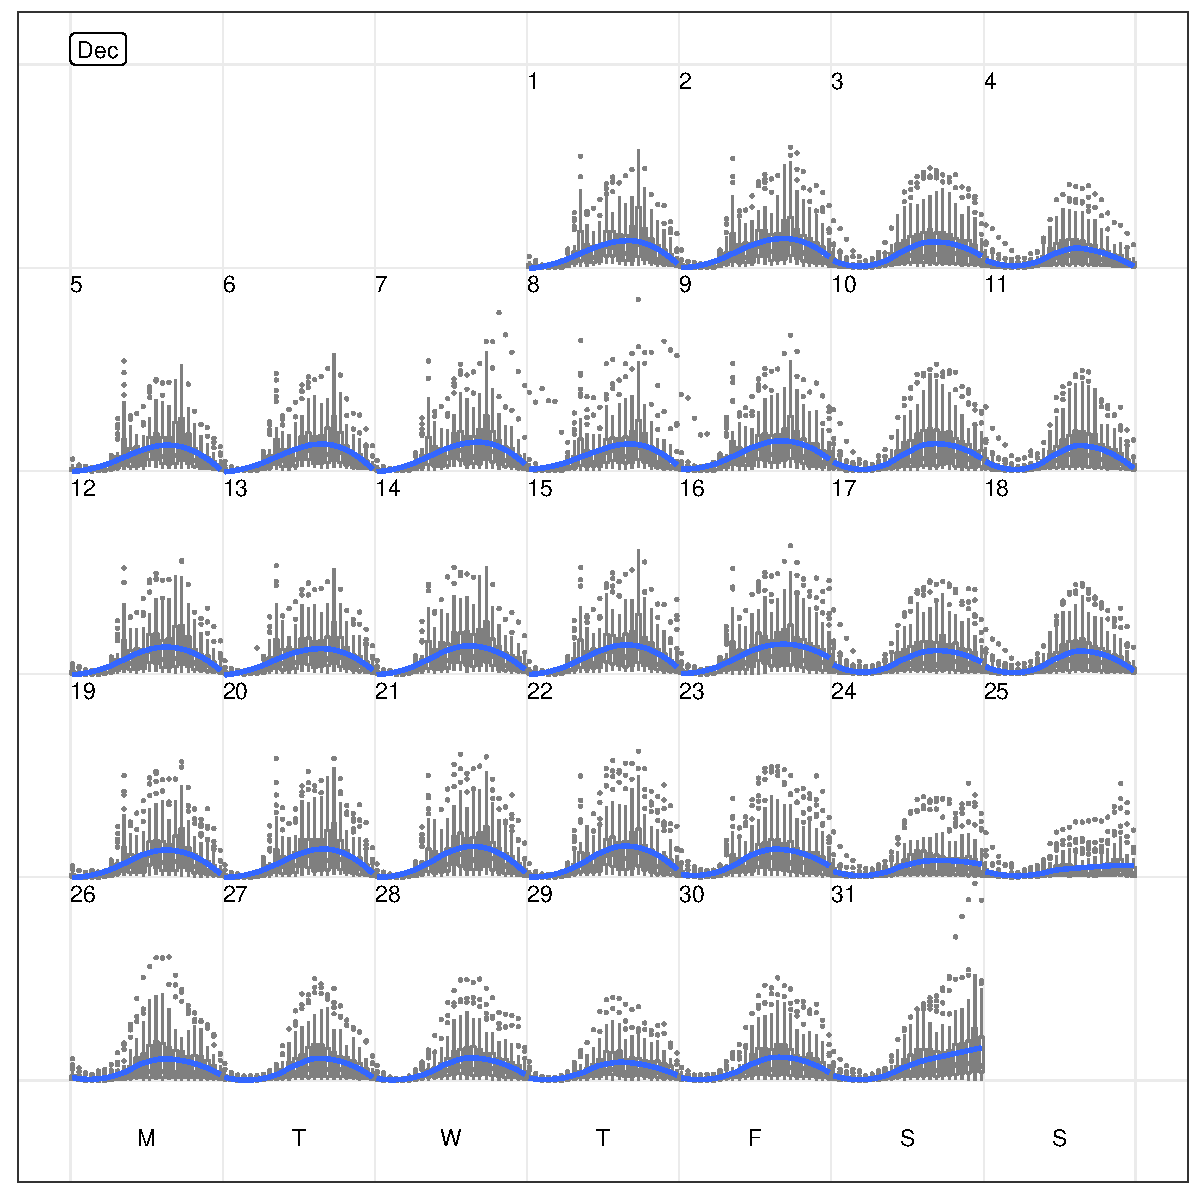
\includegraphics[width=\textwidth]{figure/boxplot-1} 

}

\caption[Side-by-side boxplot of hourly counts across all the 43 sensors in December of 2016, with the superimposing loess smooth line for each day]{Side-by-side boxplot of hourly counts across all the 43 sensors in December of 2016, with the superimposing loess smooth line for each day. It shows the hourly distribution in the city as a whole. Christmas stands out as the quietest day in December.}\label{fig:boxplot}
\end{figure}
\end{CodeChunk}

\section{Discussion}\label{discussion}

\label{sec:discussion}

The calendar-based visualisation provides data plots in the familiar (at
least for the Western world) format of an everyday tool. Special events
for the region, like Anzac Day in Australia, or Thanksgiving Day in the
USA, more easily pop out to the viewer as public holidays, rather than a
typical work day.

This sort of layout may be useful for studying consumer trends, or human
behaviour, like the pedestrian patterns. It may not work so well for
physical patterns like temperature, which are not typically affected by
human activity.

\bibliography{packages.bib,references.bib}


\end{document}

